%-------------------------
% Resume in Latex
% Author
% License : MIT
%------------------------

%---- Required Packages and Functions ----

\documentclass[a4paper,11pt]{article}
\usepackage{latexsym}
\usepackage{xcolor}
\usepackage{float}
\usepackage{ragged2e}
\usepackage[empty]{fullpage}
\usepackage{wrapfig}
\usepackage{lipsum}
\usepackage{tabularx}
\usepackage{titlesec}
\usepackage{geometry}
\usepackage{marvosym}
\usepackage{verbatim}
\usepackage{enumitem}
\usepackage[hidelinks]{hyperref}
\usepackage{fancyhdr}
\usepackage{fontawesome5}
\usepackage{multicol}
\usepackage{graphicx}
\usepackage{cfr-lm}
\usepackage[T1]{fontenc}
\setlength{\multicolsep}{0pt} 
\pagestyle{fancy}
\fancyhf{} % clear all header and footer fields
\fancyfoot{}
\renewcommand{\headrulewidth}{0pt}
\renewcommand{\footrulewidth}{0pt}
\geometry{left=1.4cm, top=0.8cm, right=1.2cm, bottom=1cm}
% Adjust margins
%\addtolength{\oddsidemargin}{-0.5in}
%\addtolength{\evensidemargin}{-0.5in}
%\addtolength{\textwidth}{1in}
\usepackage[most]{tcolorbox}
\tcbset{
	frame code={}
	center title,
	left=0pt,
	right=0pt,
	top=0pt,
	bottom=0pt,
	colback=gray!20,
	colframe=white,
	width=\dimexpr\textwidth\relax,
	enlarge left by=-2mm,
	boxsep=4pt,
	arc=0pt,outer arc=0pt,
}

\urlstyle{same}

\raggedright
\setlength{\tabcolsep}{0in}

% Sections formatting
\titleformat{\section}{
  \vspace{-4pt}\scshape\raggedright\large
}{}{0em}{}[\color{black}\titlerule \vspace{-7pt}]

%-------------------------
% Custom commands
\newcommand{\resumeItem}[2]{
  \item{
    \textbf{#1}{\hspace{0.5mm}#2 \vspace{-0.5mm}}
  }
}

\newcommand{\resumePOR}[3]{
\vspace{0.5mm}\item \hspace{1mm}
    \begin{tabular*}{0.97\textwidth}[t]{l@{\extracolsep{\fill}}r}
        \textbf{#1}\hspace{0.3mm}#2 & \textit{\small{#3}} 
    \end{tabular*}
    \vspace{-2mm}
}

\newcommand{\resumeSubheading}[4]{
\vspace{0.5mm}\item \hspace{1mm}
    \begin{tabular*}{0.98\textwidth}[t]{l@{\extracolsep{\fill}}r}
        \textbf{#1} & \textit{\footnotesize{#4}} \\
        \textit{\footnotesize{#3}} &  \footnotesize{#2}\\
    \end{tabular*}
    \vspace{-2.4mm}
}

\newcommand{\resumeProject}[4]{
\vspace{0.5mm}\item \hspace{1mm}
    \begin{tabular*}{0.98\textwidth}[t]{l@{\extracolsep{\fill}}r}
        \textbf{\parbox{0.8\linewidth}{ #1}} & \textit{\footnotesize{#3}} \\
        \footnotesize{\textit{#2}} & \footnotesize{#4}
    \end{tabular*}
    \vspace{-2.4mm}
}

\newcommand{\resumeSubItem}[2]{\resumeItem{#1}{#2}\vspace{-4pt}}

% \renewcommand{\labelitemii}{$\circ$}
\renewcommand{\labelitemi}{$\vcenter{\hbox{\tiny$\bullet$}}$}

\newcommand{\resumeSubHeadingListStart}{\begin{itemize}[leftmargin=*,labelsep=0mm]}
\newcommand{\resumeHeadingSkillStart}{\begin{itemize}[leftmargin=*,itemsep=1.7mm, rightmargin=2ex]}
\newcommand{\resumeItemListStart}{\begin{justify}\begin{itemize}[leftmargin=3ex, rightmargin=2ex, noitemsep,labelsep=1.2mm,itemsep=0mm]\small}

\newcommand{\resumeSubHeadingListEnd}{\end{itemize}\vspace{2mm}}
\newcommand{\resumeHeadingSkillEnd}{\end{itemize}\vspace{-2mm}}
\newcommand{\resumeItemListEnd}{\end{itemize}\end{justify}\vspace{-2mm}}
\newcommand{\cvsection}[1]{%
\vspace{2mm}
\begin{tcolorbox}
    \textbf{\large #1}
\end{tcolorbox}
    \vspace{-4mm}
}

\newcolumntype{L}{>{\raggedright\arraybackslash}X}%
\newcolumntype{R}{>{\raggedleft\arraybackslash}X}%
\newcolumntype{C}{>{\centering\arraybackslash}X}%
%---- End of Packages and Functions ------

%-------------------------------------------
%%%%%%  CV STARTS HERE  %%%%%%%%%%%
%%%%%% DEFINE ELEMENTS HERE %%%%%%%
\newcommand{\name}{Ervin Vavla} % Your Name
\newcommand{\course}{Electronics for RF applications} % Your Program
\newcommand{\roll}{Master's Degree in} % Your Roll No.
\newcommand{\phone}{xxx} % Your Phone Number
\newcommand{\emaila}{youremail@email.com} %Email 1
\newcommand{\emailb}{officialemail@nitw.ac.in} %Email 2



\setlength{\footskip}{5pt}
\begin{document}
\fontfamily{cmr}\selectfont
%----------HEADING-----------------


\parbox{4cm}{%
\vspace{0.6cm}
\newlength{\octradius}
\setlength{\octradius}{2cm}
\begin{tikzpicture}
  \begin{scope}
    \clip 
      (22.5:\octradius) --
      (67.5:\octradius) --
      (112.5:\octradius) --
      (157.5:\octradius) --
      (202.5:\octradius) --
      (247.5:\octradius) --
      (292.5:\octradius) --
      (337.5:\octradius) -- cycle;
    \node at (0,0) {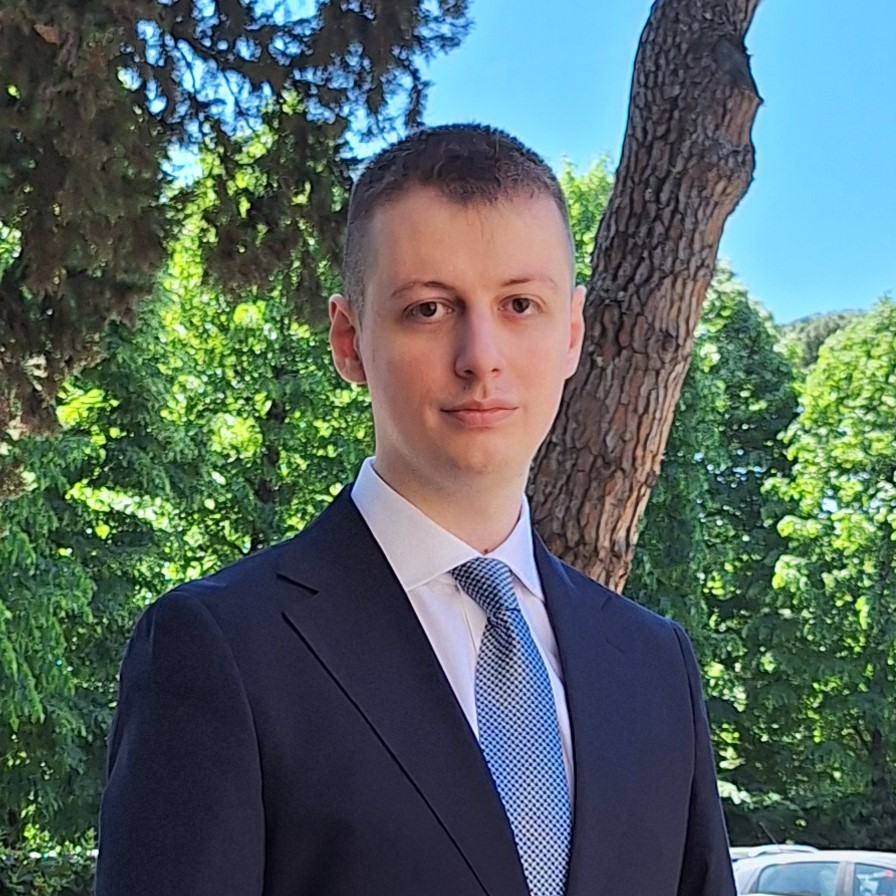
\includegraphics[width=4cm]{Foto_ErvinVavla.jpg}};
  \end{scope}

  \draw[line width=0.6pt]
      (22.5:\octradius) --
      (67.5:\octradius) --
      (112.5:\octradius) --
      (157.5:\octradius) --
      (202.5:\octradius) --
      (247.5:\octradius) --
      (292.5:\octradius) --
      (337.5:\octradius) -- cycle;
\end{tikzpicture}
}
\parbox{\dimexpr\linewidth-5cm\relax}{
\begin{tabularx}{\linewidth}{L r} \\
  \textbf{\huge \name} & {\raisebox{0.0\height}{\footnotesize \faPhone}\ +91-\phone}\\
  {\large \roll} & \href{mailto:\emaila}{\raisebox{0.0\height}{\footnotesize \faEnvelope}\ {\emaila}} \\
  \large\course &  \href{mailto:\emailb}{\raisebox{0.0\height}{\footnotesize \faEnvelope}\ {\emailb}}\\
  \textcolor{white}{Your Course} &  \href{https://yourGithubProfile.com/}{\raisebox{0.0\height}{\footnotesize \faGithub}\ {GitHub Profile}} \\
  \textcolor{white}{National Institute Of Technology, Warangal} & \href{https://www.yourLinkedinProfile.com/in/}{\raisebox{0.0\height}{\footnotesize \faLinkedin}\ {LinkedIn Profile}}
\end{tabularx}
}
% \parbox{3.0cm}{%
% \flushright \includegraphics[width=2cm,clip]{nitp_logo.png}
% }




%-----------EDUCATION-----------
\section{\textbf{Education}}
  \resumeSubHeadingListStart
    \resumeSubheading
      {University of Florence}{110/110}
      {Master's Degree in Electronics for radiofrequency applications}{09/2022-04/2026}
    \resumeSubheading
      {University of Florence}{}
      {Bachelor Degree in Electronics and Telecommunications}{09/2017-02/2022}
    \resumeSubheading
      {I.I.S Leonardo Da Vinci}{}
      {Electronics}{2013-2017}
  \resumeSubHeadingListEnd
\vspace{-5.5mm}
%



%-----------EXPERIENCE-----------------
\section{\textbf{Professional Experience}}
  \resumeSubHeadingListStart
    \resumeSubheading
      {IHP Microelectronics}{Frankfurt (Oder), Germany}
      {RF Circuit Designer -- Trainee}{05/2025--10/2025}
      \vspace{-1.0mm}
      \resumeItemListStart
        \item {Designed a D-Band (110--170 GHz) active balun in 130 nm SiGe BiCMOS technology.}
        \item {Researched the state of the art of active baluns and designed circuit topologies for D-band operation.}
        \item {Simulated and optimized amplitude balance, phase balance, gain, and power consumption.}
        \item {Prepared and optimized the integrated layout for tape-out submission.}
        \item {Prepared the measurement plan and analyzed S-parameters from .CSV files using MATLAB.}
        \vspace{2.0mm}
        \item {\textbf{Tools used}: Cadence Virtuoso, ADS, MATLAB, LaTeX, PowerPoint.}
      \resumeItemListEnd
  \resumeSubHeadingListEnd
\vspace{-8.5mm}

%-----------PROJECTS-----------------
\section{\textbf{Academic Projects}}
\resumeSubHeadingListStart

    \resumeProject
      {VHDL for Real-Time Reconfiguration of the Operating Frequency of a PLL in an FPGA}
      {Design and simulation of a VHDL-based digital control system for FPGA applications.}
      {02/2022}
      {Florence, Italy}
      \vspace{-1.0mm}
      \resumeItemListStart
        \item {Designed VHDL modules for real-time control of the PLL operating frequency.}
        \item {Simulated and verified the design using ModelSim.}
        \item {Implemented and tested the project using Intel Quartus on an FPGA development board.}
        \vspace{2.0mm}
        \item {\textbf{Tools used}: Intel Quartus, ModelSim, PowerPoint.}
      \resumeItemListEnd
      \vspace{-2mm}
    
\resumeSubHeadingListEnd
\vspace{-5.5mm}



%-----------Technical skills-----------------
\section{\textbf{Technical Skills and Interests}}
 \begin{itemize}[leftmargin=0.05in, label={}]
  \vspace{1mm}
    \small{\item{
     \textbf{Programming Languages}{: MATLAB, C} \\[1.5pt]
     \textbf{EDA and Simulation Tools}{: ADS, Cadence Virtuoso, LTspice} \\[1.5pt]
     \textbf{Technical Skills}{: Analog Circuit Design, RF/mm-Wave Circuit Design, S-Parameter Analysis, IC Layout} \\[1.5pt]
     \textbf{Documentation Tools}{: LaTeX, PowerPoint} \\[1.5pt]
     \textbf{Areas of Interest}{: Analog Circuit Design, RF/mm-Wave Circuit Design, Integrated Circuits (IC), RFIC Design} \\
    }}
 \end{itemize}
 \vspace{-16pt}

 %-----------LANGUAGE-----------------
\section{\textbf{Languages}}
 \begin{itemize}[leftmargin=0.05in, label={}]
  \vspace{1mm}
\small{\item{
     \textbf{Italian}{: Fluent} \\[1.5pt]
     \textbf{English}{: Excellent reading, good written and spoken communication} \\[1.5pt]
     \textbf{Albanian}{: Basic spoken communication}
    }}
 \end{itemize}
 \vspace{-16pt}


\begin{comment}
%-----------Positions of Responsibility-----------------
\section{\textbf{Positions of Responsibility}}
\vspace{-0.4mm}
\resumeSubHeadingListStart
\resumePOR{Position, } % Position
    {Club or Event} %Club,Event
    {Position tenure} %Tenure Period
\resumePOR{Position, } % Position
    {Club or Event} %Club,Event
    {Position tenure} %Tenure Period
\resumeSubHeadingListEnd
\vspace{-5mm}
\end{comment}

\begin{comment}
  %-----------Achievements-----------------
\section{\textbf{Achievements}}
\vspace{-0.4mm}
\resumeSubHeadingListStart
\resumePOR{Achievement } % Award
    {description} % Event
    {Event dates} %Event Year
    
\resumePOR{Achievement } % Award
    {description} % Event
    {Event dates} %Event Year
\resumeSubHeadingListEnd
\vspace{-5mm}
%-------------------------------------------
\end{comment}
\end{document}
